\documentclass{report}
\usepackage[T1]{fontenc} % Fontes T1
\usepackage[utf8]{inputenc} % Input UTF8
\usepackage[backend=biber, style=ieee]{biblatex} % para usar bibliografia
\usepackage{csquotes}
\usepackage[portuguese]{babel} %Usar língua portuguesa
\usepackage{blindtext} % Gerar texto automaticamente
\usepackage[printonlyused]{acronym}
\usepackage{hyperref} % para autoref
\usepackage{graphicx}
\usepackage{indentfirst}
\usepackage{float}
\usepackage{geometry}

\geometry{
    paper=a4paper,
    margin=45pt,
    includefoot
}

\bibliography{bibliografia}


\begin{document}
%%
% Definições
%
\def\titulo{Máquina de Pão}
\def\data{DATA}
\def\autores{Tiago Garcia, José Fernandes}
\def\autorescontactos{(114184) tiago.rgarcia@ua.pt, (114472) jbfernandes@ua.pt}
\def\versao{VERSAO 1}
\def\departamento{Dept. de Eletrónica, Telecomunicações e Informática}
\def\empresa{Universidade de Aveiro}
%
%%%%%% CAPA %%%%%%
%
\begin{titlepage}

\begin{center}
%
\vspace*{50mm}
%
{\Huge \titulo}\\ 
%
\vspace{10mm}
%
{\Large \empresa}\\
%
\vspace{10mm}
%
{\LARGE \autores}\\ 
%
\vspace{30mm}
%
\begin{figure}[h]
\center

\includegraphics{../images/ua}\label{fig:ua-logo}
\end{figure}
%
\vspace{30mm}
\end{center}
%
\begin{flushright}
\versao
\end{flushright}
\end{titlepage}

%%  Página de Título %%
\title{%
{\Huge\textbf{\titulo}}\\
{\Large \departamento\\ \empresa}
}
%
\author{%
    \autores \\
    \autorescontactos
}
%
\date{\today}
%
\maketitle

\pagenumbering{roman}

\tableofcontents
\listoftables     % descomentar se necessário
\listoffigures    % descomentar se necessário


%%%%%%%%%%%%%%%%%%%%%%%%%%%%%%%
\clearpage
\pagenumbering{arabic}

%%%%%%%%%%%%%%%%%%%%%%%%%%%%%%%%
\chapter{Introdução}
\label{ch:introducao}

Como projeto final da cadeira de \ac{lsd} foi-nos proposto o projeto da máquina de pão automática.

Para tal, usamos \ac{vhdl} para simular o seu comportamento na placa FPGA Terasic DE2-115.\ Haverão 3 secções de displays, uma para o tempo do programa, outra para o tempo extra e outra para o atraso até ao ínicio da execução do programa.\ Haverá também um interruptor para selecionar o programa a ser executado, 7 interruptores para escolher o atraso inicial (introduzido em binário) e ainda 3 butões, o `Start/Stop', outro para reiniciar a máquina e o último para adicionar o possível tempo extra.\\

\chapter{Manual de Utilização}
\label{ch:manual-de-utilizacao}
\section{Programas}
\label{sec:programas}

\begin{table}[H]
    \centering
    \label{tab:programas}
    \begin{tabular}{|c|c|}
        \hline Pão Caseiro & Pão Rústico \\ \hline
        \begin{tabular}{c|c}
            Fase da Fabricação & Tempo (segundos) \\
            Amassar & 10 \\
            Levedar & 4 \\
            Cozer & 10 \\
        \end{tabular}
        &
        \begin{tabular}{c|c}
            Fase da Fabricação & Tempo (segundos) \\
            Amassar & 15 \\
            Levedar & 8 \\
            Cozer & 10 \\
        \end{tabular} \\ \hline
    \end{tabular}
    \caption{Programas de Pão}
\end{table}

\section{Funcionamento}
\label{sec:funcionamento}

A máquina inicializa permitindo o utilizador selecionar o programa a ser executado.\ Para tal, deve colocar o interruptor `Selecionador Programa' na posição do programa que deseja.\ O `Pão Caseiro' será a posição inicial do interruptor e o `Pão Rústico' será a outra posição.\ Sempre que a máquina é reiniciada estas posições são reatribuídas.\ Os programas, bem como as suas durações, são descritos em cima: Tabela~\ref{tab:programas}.

O utilizador pode também escolher o atraso inicial a ser aplicado e, para isso, terá de usar os 7 interruptores do `Selecionador Atraso' para indicar o número, este terá de ser introduzido em binário e a máquina irá converter para decimal.\ Este valor poderá variar entre 0 e 90 segundos e qualquer valor superior a isso será interpretado como 90.

Após a seleção do programa e do atraso inicial o utilizador poderá clicar no botão `Start/Stop' para iniciar a máquina.\ O programa irá começar assim que o atraso inicial chegar a 0.\ Poderá ver a fase em que o programa se encontra com os `LEDS Display Fase':
\begin{itemize}
    \item 3 LEDS ligados $\rightarrow$ Amassar
    \item 2 LEDS ligados $\rightarrow$ Levedar
    \item 1 LED ligado~~~~$\rightarrow$ Cozer ou Tempo Extra
    \item 0 LEDS ligados $\rightarrow$ Standby, Atraso Inicial ou Espera da Confirmação do Tempo Extra/Reinicialização
\end{itemize}

O tempo, tanto do atraso como da programação normal poderá ser pausado e continuado em qualquer momento ao longo da sua execução.

Após o final da programação normal o utilizador terá a possibilidade de adicionar tempo extra utilizando o botão `Tempo Extra'.\ Para iniciar o mesmo, o utilizador deverá clicar no botão `Start/Stop'.\ Tal como o atraso inicial e o tempo do programa, o tempo extra também poderá ser pausado e continuado em qualquer momento.\ Se o botão de `Start/Stop' for pressionado com o tempo extra a 0 então a máquina irá ser reiniciada.\ O utilizador pode usar o tempo extra o número de vezes que desejar.

O `LED Display Execução' estará ligado durante a execução do programa normal e do tempo extra.

A máquina poderá também ser reinicada em qualquer momento usando o botão `Reset'.

\section{Esquema da Máquina}
\label{sec:esquema-da-maquina}

\begin{figure}[H]
    \center
    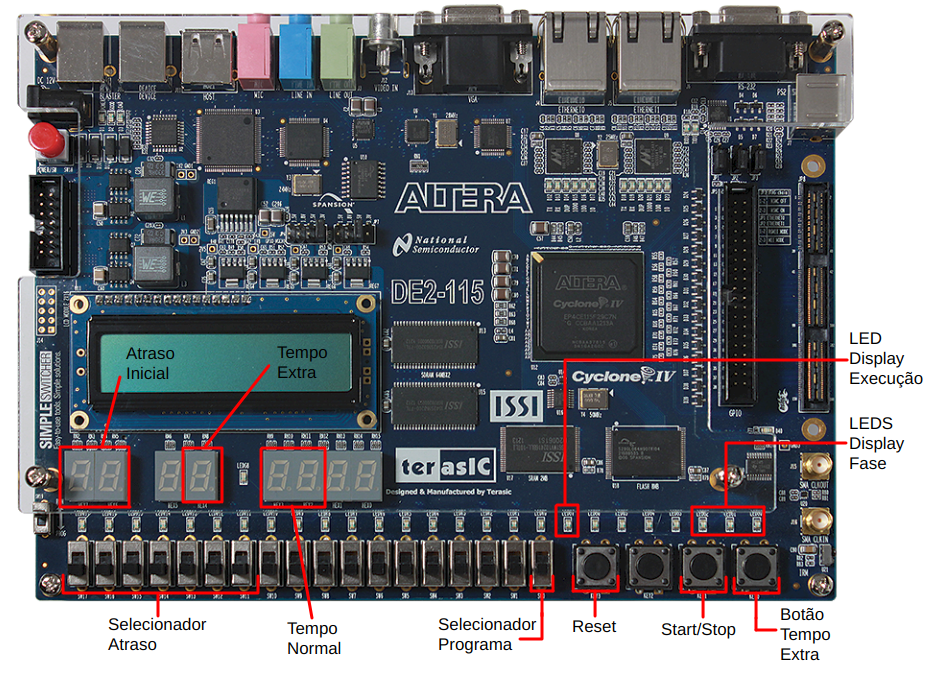
\includegraphics[scale=.4]{../images/esquema-placa}\caption{Ilustração do Esquema da Máquina}
    \label{fig:esquema-placa}
\end{figure}

\begin{itemize}
    \item \textbf{Display: Atraso Inicial} $\rightarrow$ Display para mostrar o tempo que irá decorrer antes do início da execução do programa.
    \item \textbf{Display: Tempo Extra} $\rightarrow$ Display para mostrar o tempo extra do programa.
    \item \textbf{Display: Tempo Programa} $\rightarrow$ Display para mostrar o tempo de execução do programa.
    \item \textbf{LED: Display Execução} $\rightarrow$ LED para indicar que o programa está a ser executado.
    \item \textbf{LEDS: Display Fases} $\rightarrow$ LEDS para indicar a fase do programa que está a ser executada.
    \item \textbf{Switch: Selecionador Atraso} $\rightarrow$ Série de interruptores para selecionar o tempo de atraso inicial.
    \item \textbf{Switch: Selecionador Programa} $\rightarrow$ Interruptor para selecionar o programa a ser executado.
    \item \textbf{Botão: Reset} $\rightarrow$ Botão para reiniciar a máquina.
    \item \textbf{Botão: `Start/Stop'} $\rightarrow$ Botão para iniciar ou parar a execução do programa.
    \item \textbf{Botão: Tempo Extra} $\rightarrow$ Botão para adicionar tempo extra ao programa.
\end{itemize}

\chapter{Arquitetura e Implementação}
\label{ch:arquitetura-e-implementacao}
O Top-Level da máquina é composto por 3 componentes principais que depois se ramificam em subcomponentes mais pequenos.

A figura~\ref{fig:top-level} representa uma ilustração gráfica do Top-Level da máquina implementado em \ac{vhdl}.

\begin{figure}[h]
    \center
    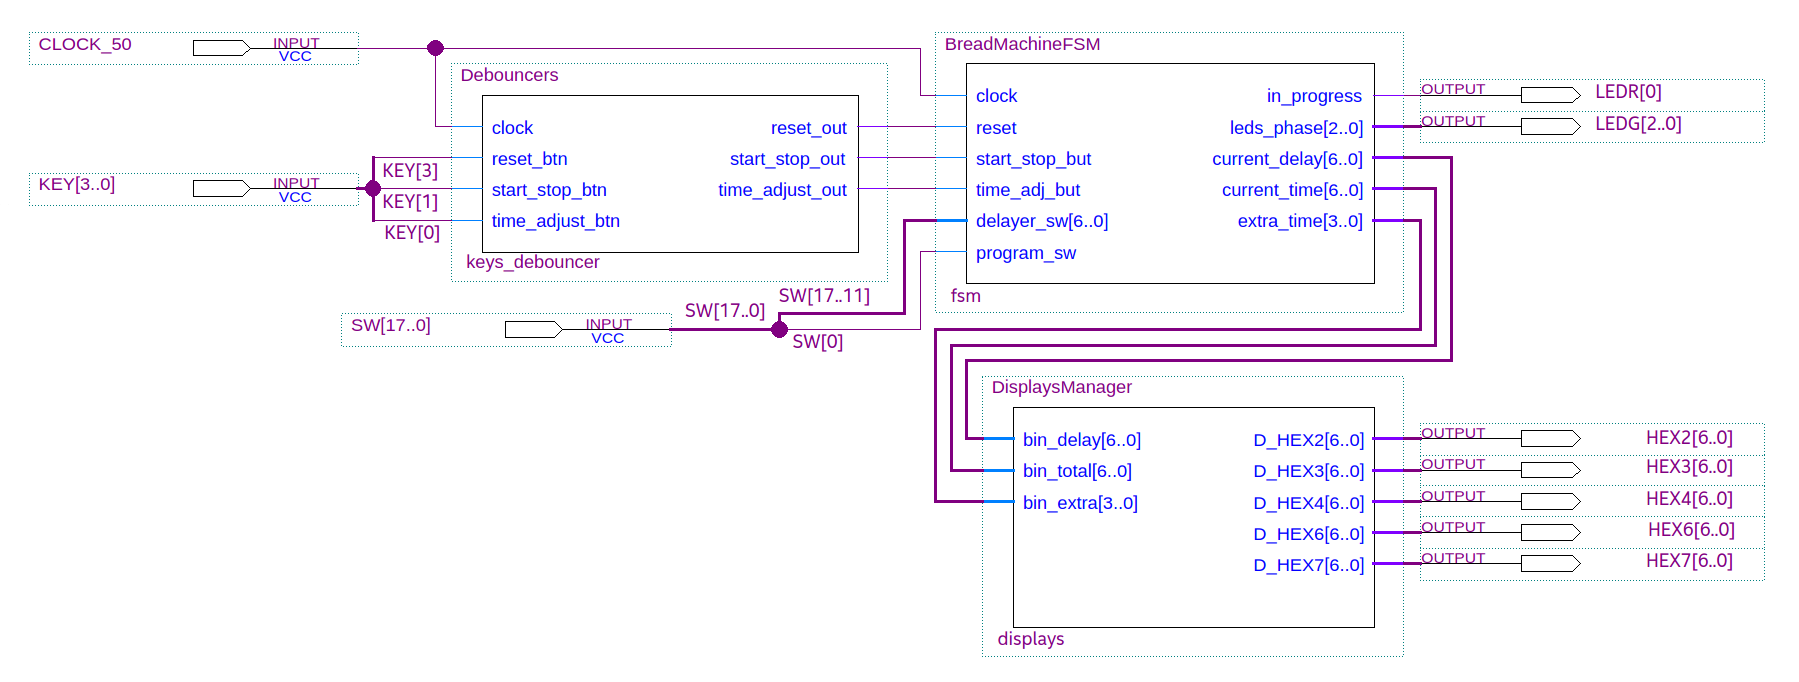
\includegraphics[scale=.25]{../images/top-level-design}\caption{Ilustração do Top-Level da Máquina}
    \label{fig:top-level}
\end{figure}

\section{Debouncers}
\label{sec:debouncers}
Este componente é responsável por fazer o Debounce dos botões.\ Isto é necessário pois quando um botão é pressionado gera centenas de sinais, o que pode muitas vezes causar problemas.

O bloco recebe o valor do relógio geral da máquina bem como os valores dos botões a ser afetados.

Dentro do bloco os valores dos botões são distribuídos entre 3 debouncers onde são processados para gerar os sinais pretendidos.

Sai deste bloco os sinais dos botões já corrigidos para que seja emitido apenas 1 sinal positivo por clique.

\section{BreadMachineFSM}
\label{sec:fsm}
Este é o componente principal da máquina e é o responsável pelo processamento do funcionamento da mesma.

Entram neste componente o sinal do relógio da máquina, os sinais dos botões de `Reiniciar', `Start/Stop' e `Tempo Extra', recebe também o sinal do interruptor do `Selecionador Programa' e, por último, o valor do vetor gerado pelos interruptores do `Selecionador Atraso'.

Como saídas irá ter o sinal para indicar se a máquina se encontra no estado `Progress' ou `Extra'.\ Faz também parte das saídas o vetor de indicação da `Fase da Fabricação' que está a decorrer no momento.\ Estas saídas são diretamente ligadas aos LEDS da máquina: 1 LED vermelho e 3 LEDS verdes, respetivamente.

O funcionamento da máquina de estados será descrito com recurso à figura~\ref{fig:state-machine}.

\pagebreak

\begin{figure}
    \centering
    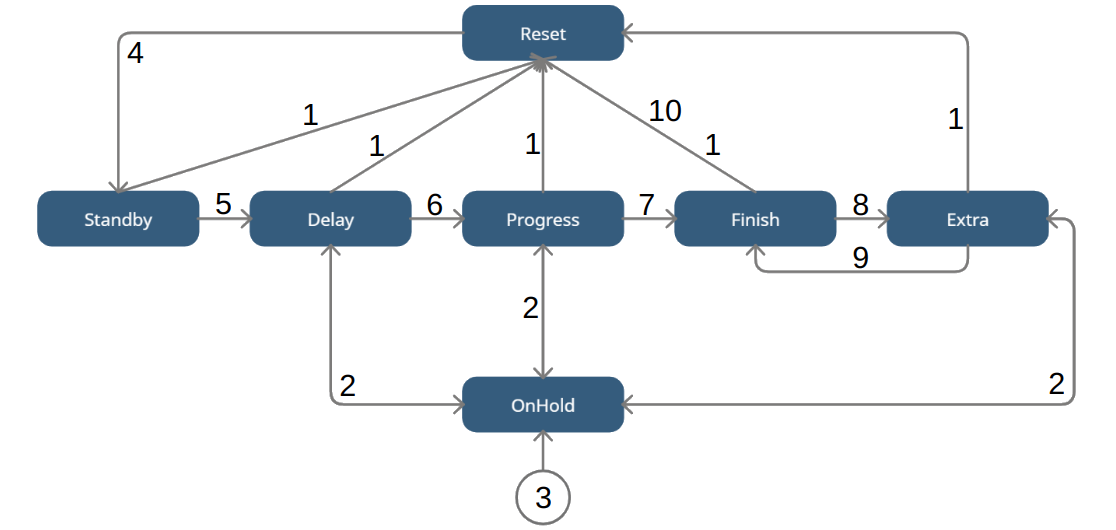
\includegraphics[scale=.4]{../images/state-machine}
    \caption{Esquema da Máquina de Estados}
    \label{fig:state-machine}
\end{figure}

\begin{enumerate}
    \item \textbf{Reset}
        \\$\hookrightarrow$ A máquina volta sempre ao estado de Reset quando o botão `Reset' é pressionado.
    \item \textbf{(Delay/Progress/Extra) $\leftrightarrow$ OnHold}
        \\$\hookrightarrow$ Quando o botão de `Start/Stop' é utilizado e o estado é `Delay', `Progress' ou `Extra', muda o estado para `OnHold' para pausar a máquina.
        \\$\hookrightarrow$ Quando o botão de `Start/Stop' é utilizado e o estado atual é `OnHold', retoma o estado para o qual a máquina se previamente encontrava (`Delay', `Progress' ou `Extra').
    \item \textbf{OnHold $\rightarrow$ OnHold}
        \\$\hookrightarrow$ Atualiza o valor do start\_stop negando o mesmo.\ Fica neste estado enquanto o valor do start\_stop for `0' e sai do estado quando passar para `1'.
    \item \textbf{Reset $\rightarrow$ Standby}
        \\$\hookrightarrow$ Assim que a máquina é reiniciada, o estado muda automaticamente para Standby após a reinicialização de todos os valores.
    \item \textbf{Standby $\rightarrow$ Delay}
        \\$\hookrightarrow$ Quando o botão de `Start/Stop' é pressionado, muda de estado para `Delay' começando o timer do atraso inicial com o valor escolhido.
    \item \textbf{Delay $\rightarrow$ Progress}
        \\$\hookrightarrow$ Assim que o tempo do atraso inicial chegar a 0, o estado passa automaticamente de `Delay' para `Progress'.
    \item \textbf{Progress $\rightarrow$ Finish}
        \\$\hookrightarrow$ Assim que o tempo da programação chegar a 0, o estado passa automaticamente de `Progress' para `Finish'.
        \\$\hookrightarrow$ Neste estado, a máquina não se encontra com nenhuma mudança visual imediata, fica a aguardar por um dos botões.\ Usando o botão `Tempo Extra' poderá ser definido o tempo extra a aplicar à máquina posteriormente no estado `Extra'.
    \item \textbf{Finish $\rightarrow$ Extra}
        \\$\hookrightarrow$ Esta mudança é realizada quando o botão `Start/Stop' é pressionado e o tempo extra não se encontra a 0.
    \item \textbf{Extra $\rightarrow$ Finish}
        \\$\hookrightarrow$ Assim que o tempo do tempo extra chegar a 0, o estado passa automaticamente de `Extra' para `Finish'.
    \item \textbf{Finish $\rightarrow$ Reset}
        \\$\hookrightarrow$ Esta mudança é realizada quando o botão `Start/Stop' é pressionado e o tempo extra encontra-se a 0.\ Este passo reinicializa a máquina automaticamente.
\end{enumerate}

\textbf{Nota:} Os passos 2, 3, 8 e 9 podem ocorrer um número de vezes indefinido durante uma execução completa da máquina.

\section{DisplaysManager}
\label{sec:displays-manager}
Este último componente é o responsável pela gestão dos displays para que os números dos tempos da máquina sejam corretamente visualizados.

O bloco recebe separadamente os valores dos 3 tempos: `Atraso Inicial', `Tempo Normal' e `Tempo Extra'.

O tempo extra é diretamente processado para a codificação dos displays, enquanto que o atraso inicial e o tempo normal têm de ser convertidos em numeração decimal (gerando 2 valores cada) para depois serem codificados.\ Este passo produz 5 valores diferentes.

Esses 5 valores são então distribuídos pelos 5 displays da máquina.

\chapter{Validações}
\label{ch:validacoes}
No decorrer do nosso projeto fomos confrontados com diversas adversidades no que toca a simulação e validação.\ Como tal, a principal maneira de verificação foi prática e feita com a placa, já que o trabalho funciona maioritariamente em segundos, um tempo dificil de se trabalhar tanto no simulador, como na testbench.

\chapter{Conclusões e Contribuições}
\label{ch:conclusoes-e-contribuicoes}

\section{Conclusões}
\label{sec:conclusoes}
Após uma breve reflexão observámos que com este trabalho foram desenvolvidas novas capacidades em VHDL, lógica de estruturação (aplicada durante o planeamento das funções), otimização (de forma a simplificar o trabalho da melhor forma possivel) e ainda capacidades a nível de trabalho em grupo.\ Vimos também algumas das capacidades da placa e o potencial da disciplina, o que nos despertou interesse em saber mais e talvez desenvolver algo por conta própria.\ No geral, foram cumpridos todos os objetivos requeridos e ainda foram implementadas novas funcionalidades.

Autoavaliamos o nosso trabalho com 18 valores.

\section{Contribuições dos autores}
\label{sec:contribuicoes-dos-autores}
Neste projeto, ambos os elementos do grupo trabalharam de igual forma e com semelhante nível de empenho e por isso cada elemento do grupo tem uma percentagem de participação de 50\%.

%%%%%%%%%%%%%%%%%%%%%%%%%%%%%%%%%
\chapter*{Acrónimos}
\begin{acronym}
    \acro{ua}[UA]{Universidade de Aveiro}
    \acro{leci}[LECI]{Licenciatura em Engenharia de Computadores e Informática}
    \acro{lsd}[LSD]{Laboratório de Sistemas Digitais}
    \acro{vhdl}[VHDL]{VHSIC Hardware Description Language}
\end{acronym}


%%%%%%%%%%%%%%%%%%%%%%%%%%%%%%%%%
\printbibliography

\end{document}
